\documentclass[11pt]{beamer}
\usetheme{Montpellier}
\usefonttheme[onlymath]{serif}
\usecolortheme{rose}

\usepackage{tikz} \usepackage{graphicx} \usepackage{algorithm} \usepackage[noend]{algpseudocode} \usepackage{caption}
\usepackage{amsmath} \usepackage{pgfplots} \usepackage{float}
%\usepackage{graphicx} \usepackage{url} \usepackage{hyperref}  \usepackage{amsmath}
%\usepackage{amssymb} \usepackage{array} \usepackage{listings} \usepackage{color} \usepackage{textcomp}
%\usepackage[utf8]{inputenc} \usepackage{natbib} \usepackage{algorithm}
%\usepackage[noend]{algpseudocode} \usepackage{csquotes} \usepackage{mathtools}

\usetikzlibrary{shapes.geometric, arrows}

\setbeamertemplate{navigation symbols}{}
\setbeamerfont{page number in head/foot}{size=\fontsize{9}{11}}
\setbeamertemplate{footline}[frame number]
\setbeamertemplate{section in toc}{\inserttocsectionnumber.~\inserttocsection}

\author{Glenn Galvizo}
\title{MCMC ABC for Microsatellite Mutation Models}
\institute{University of Hawaii at Manoa}

\begin{document}
    \begin{frame}
        \titlepage
    \end{frame}

	\section{Introduction}\label{sec:introduction}
	\begin{frame}
		\frametitle{Overview}
        \tableofcontents
	\end{frame}

	\begin{frame}
		\frametitle{How much do we know about human history?}
	\end{frame}

	\subsection{Problem Statement}\label{subsec:problemStatement}
	\begin{frame}
		\frametitle{Research Goal: Verification}
	\end{frame}

	\section{Background}\label{sec:background}
	\subsection{Microsatellites}\label{subsec:microsatellites}
    \begin{frame}

    \end{frame}

    \subsection{Microsatellite Mutation}\label{subsec:microsatelliteMutation}
    \begin{frame}
        \pgfplotsset{compat=1.5}
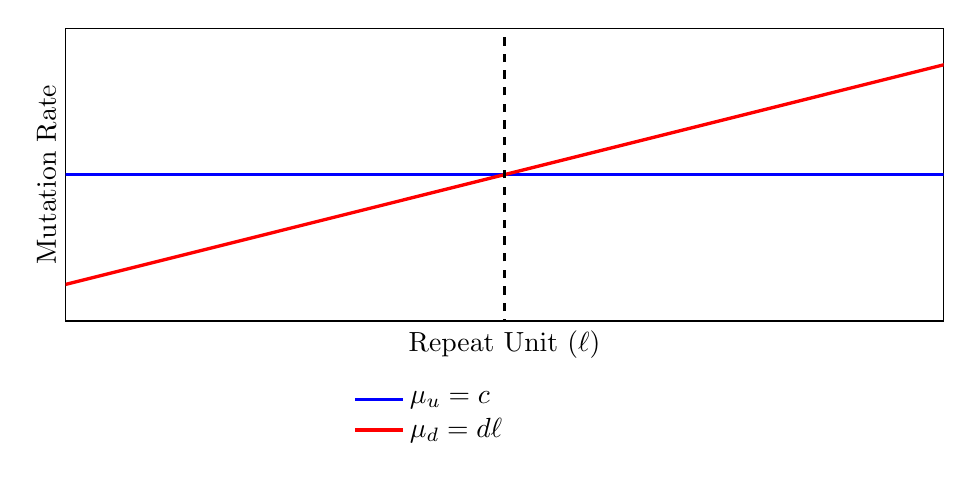
\begin{tikzpicture}
    \begin{axis}[
    width=1.05\linewidth, height=5.3cm,
    ylabel={Mutation Rate}, ymin=0.01, ymax=0.05,
    xlabel={Repeat Unit ($\ell$)}, xmin=6, xmax=18,
    xtick={0, 2, 4, 6, 8, 10, 12, 14, 16, 18, 20, 22, 24},
    samples=100, no markers, enlargelimits=false, legend style={at={(0.5,-0.2)},anchor=north,draw=none},
    legend cell align={left}, domain=0:25, ticks=none
    ]
        \addplot+[very thick]{0.03};
        \addlegendentry{$\mu_u = c$};

        \addplot+[very thick] {0.0025*x};
        \addlegendentry{\vspace*{5em}$\mu_d = d\ell$ \hspace*{5em}};

        \addplot+[very thick, black, dashed, forget plot] coordinates {(12, 0) (12, 0.05)};
    \end{axis}
\end{tikzpicture}
    \end{frame}

    \section{Methodology}\label{sec:methodology}
	\subsection{Backwards Simulation}\label{subsec:backwardsSimulation}
    \begin{frame}

    \end{frame}

    \subsection{Approximate Bayesian Computation}\label{subsec:approximateBayesianComputation}
    \begin{frame}

    \end{frame}

	\subsection{Monte Carlo Markov Chain (MCMC)}\label{subsec:monteCarloMarkovChainmcmc}
    \begin{frame}

    \end{frame}

    \section{Results}\label{sec:results}
    \begin{frame}

    \end{frame}

    \subsection{$u$ Upward Linear Bias Parameter}\label{subsec:upwardLinearBiasParameter}
    \begin{frame}

    \end{frame}

    \subsection{$d$ Downward Linear Bias Parameter}\label{subsec:downwardLinearBiasParameter}
    \begin{frame}

    \end{frame}

    \subsection{$c$ Upward Constant Bias Parameter}\label{subsec:upwardConstantBiasParameter}
    \begin{frame}

    \end{frame}

    \section{Conclusion}\label{sec:conclusion}
    \begin{frame}
        
    \end{frame}

    \begin{frame}
        \frametitle{Acknowledgments}
        \begin{itemize}
            \item Dr. Floyd Reed \medskip
            \item Undergraduate Showcase \medskip
            \item The Audience \medskip
        \end{itemize}
    \end{frame}

    \begin{frame}
        \centering{\huge{Questions?}}
    \end{frame}


%	\section{Microsatellites}\label{sec:microsatellites}
%	\begin{frame}
%		\frametitle{What are microsatellites?}\medskip
%
%		\begin{definition}
%			\emph{Microsatellites} (or SSRs) are repetitive DNA motifs (2-10 nucleotides), which are repeated in tandem
%		\end{definition}\bigskip
%
%		\begin{enumerate}
%			\item Mutate in terms of repeat units, not single nucleotides
%			\item Mutate more often than point mutations
%			\item Interested in number of repeats (repeat units)
%		\end{enumerate}\bigskip\bigskip
%
%		\centering{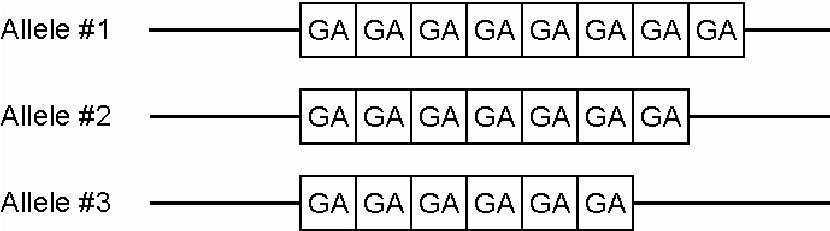
\includegraphics[scale=0.3]{images/microsatellite-ga.png}}
%	\end{frame}
%
%	\section{Data}\label{sec:data}
%	\begin{frame}
%		\frametitle{What data are we using?}\bigskip
%
%		\begin{enumerate}
%			\item Focusing on $GATA$ motifs
%			\item Collected 330 different populations of SSRs from ALFRED
%			\item Each typed population has sample size $n$, a repeat length, and associated frequency
%		\end{enumerate}\bigskip
%
%		\centering{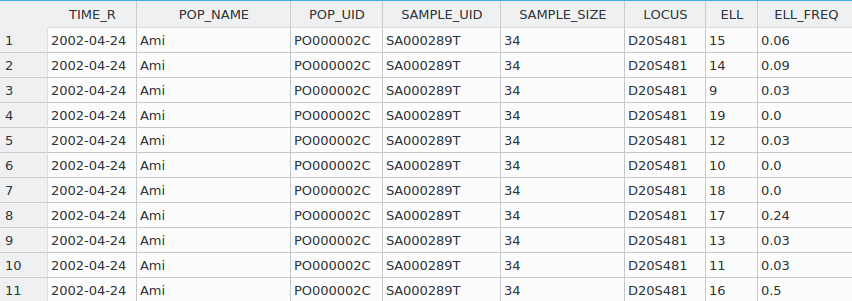
\includegraphics[scale=0.45]{images/ami-pop.png}}
%	\end{frame}
%
%	\section{Mutation Model}\label{sec:mutationModel}
%	\begin{frame}
%		\frametitle{Modeling Mutation}
%		\begin{enumerate}
%			\item Common ancestor of length $i_0$ \smallskip
%			\item Current generation composed of alleles from previous generation \smallskip
%			\item Random mating, constant sized population of $2N$ alleles \smallskip
%			\item Want all resulting alleles to share common ancestor \smallskip
%			\item After this, sample $n$ alleles randomly from simulation and compare to data \smallskip
%		\end{enumerate}
%	\end{frame}
%
%	\subsection{Number of Repeat Units}\label{subsec:numberOfRepeatUnits}
%	\begin{frame}
%		\frametitle{How many repeat units are gained / lost per mutation?}
%		\begin{block}{Two-Phase Model (TPM)}
%			\begin{itemize}
%				\item $\pm 1$ repeat unit with probability $p$
%				\item $\pm \geq 1$ repeat units with probability $1 - p$, distributed by $\gamma(m)$
%			\end{itemize}
%		\end{block}\bigskip
%
%		$\gamma(m)$ represents a truncated geometric distribution, sampled using:
%		\begin{equation}
%			\left\lfloor \frac{\log\left( 1 - X(1 - (1 - m)^{\Omega - \kappa})\right)}{\log(1 - m)}  \right\rfloor
%			+ \kappa
%		\end{equation}
%		where $X\sim U(0, 1)$ represents some uniform random variable, $m = $ success probability,
%		and $[\kappa, \Omega]$ represent the lower and upper bounds of our repeat lengths.
%	\end{frame}
%
%	\subsection{Mutation Rates}\label{subsec:mutationRates}
%	\begin{frame}
%		\frametitle{How often do mutations occur?}
%		\begin{block}{Proportional Slippage Model (PS)}
%			\begin{itemize}
%				\item Strength of length dependence determined by $s \in (-1 / (\Omega - \kappa + 1), \ \infty)$
%			\end{itemize}
%		\end{block}\bigskip
%
%		Mutation rate $\beta(i, s)$ determined by:
%		\begin{equation}
%			\beta(i, s) = \mu (1 + (i - \kappa)s)
%		\end{equation}
%		where $\mu \in [0, 1]$ represents a constant mutation rate and $i \in [\kappa, \Omega]$ represents the
%		repeat length of some allele.
%	\end{frame}
%
%	\subsection{Contractions or Expansions}\label{subsec:contractionsOrExpansions}
%	\begin{frame}
%		\frametitle{When do contractions / expansions occur?}
%		\begin{block}{Proportional Slippage Model (PS), continued}
%			\begin{itemize}
%				\item Mutate toward focal bias $f = ((u - 0.5) / v) + \kappa$ when $0.5 < u < 1$ and
%				$(u - 0.5) / (\Omega - \kappa) < v < \infty$
%			\end{itemize}
%		\end{block}\bigskip
%
%		The probability of an expansion $\alpha(u, v, i)$, which is also dependent on the repeat length:
%		\begin{equation}
%			\alpha(u, v, i) = \mathit{max}(0, \ \mathit{min}(1, \ u - v(i - \kappa)))
%		\end{equation}
%		where $u \in [0, 1]$ represents some constant bias and $v \in (-\infty, \infty)$ represents the linear bias
%		parameter (toward our focal length).
%	\end{frame}
%
%	\section{Simulation}\label{sec:simulation}
%	% https://qph.fs.quoracdn.net/main-qimg-63b52ff85dd6b1cc2040236734a92b4a
%	\subsection{Coalescence Based}\label{subsec:coalescenceTheoryBased}
%	\begin{frame}
%		\frametitle{Coalescence Based Simulation}
%		\begin{columns}
%			\begin{column}{0.5\textwidth}
%				\centering{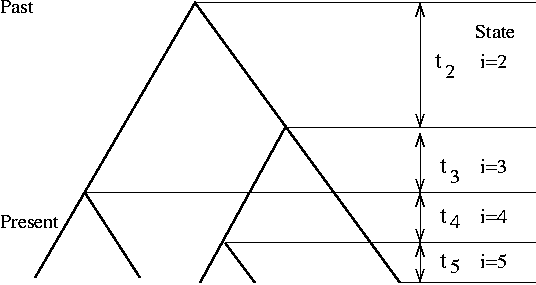
\includegraphics[scale=0.3]{images/coalescence.png}}\\ \medskip
%				\tiny{
%					\begin{enumerate}
%						\item Generate 2 individuals $i_1^{(1)}, i_1^{(2)}$ from common ancestor $i_0$
%						\item Generate 3 individuals $i_2^{(1)}, i_2^{(2)}, i_2^{(3)}$ from previous generation
%						\item[$\vdots$]
%						\item[$2N - 1$.] \medskip Generate $2N$ individuals from previous generation
%					\end{enumerate}
%				}
%			\end{column}
%			\begin{column}{0.5\textwidth}
%				\begin{enumerate}
%					\item Define parameters $(i_0, N, \mu, s, \kappa, \omega, u, v, m, p)$
%					\item Simulate forward, start from common ancestor
%					\item Time until $j$ individuals coalesce $t_j = \frac{2N}{C(j, 2)}$
%					\item Guarantees that all members of end population coalesce, requires only $2N$ iterations,
%					requires less memory
%				\end{enumerate}
%			\end{column}
%		\end{columns}
%	\end{frame}
%
%	\newcommand{\set}[1]{\{#1\}}
%	\subsection{The Algorithm}\label{subsec:theAlgorithm}
%	\begin{frame}
%		\frametitle{The Algorithm}
%		\begin{algorithmic}[1]
%			\Procedure{Evolve}{}
%				\State $\ell \gets \set{i_0}$
%				\For{$j = 1 \text{\textbf{ to }} 2N$} \Comment Repeat until $2N$ alleles exist
%					\State $\ell_j \gets \emptyset$
%					\For{$C(j, 2)$ times} \Comment All of current population.
%						\State $i \gets $ some allele from $\ell$
%						\For{$2N / C(j, 2)$} \Comment Time to coalescence.
%							\State $y_1 \gets 1$ dependent on: $\beta(i, s)$, else $0$
%							\State $y_2 \gets 1$ dependent on: $\alpha(u, v, i)$, else $-1$
%							\State $y_3 \gets 1$ dependent on: $p$, else  $\sim \gamma(m)$
%							\State $i \gets i + y_1 \cdot y_2 \cdot y_3$
%						\EndFor
%						\State $\ell_j \gets \set{i} \cup \ell_j$
%					\EndFor
%					\State $\ell \gets \ell_j$ \Comment Replace old ancestors with new ones.
%				\EndFor
%				\State \textbf{return} $\ell$
%			\EndProcedure
%		\end{algorithmic}
%	\end{frame}
%
%	\section{Future Work}\label{sec:futureWork}
%	\begin{frame}
%		\frametitle{Future Work}
%		\begin{enumerate}
%			\item Markov chain monte carlo (MCMC) to estimate parameters \smallskip
%			\item Work with multiple common ancestors \smallskip
%			\item Work with multiple populations converging and separating \smallskip
%			\item Fix mutation model parameters and estimate $N$ \smallskip
%		\end{enumerate}
%	\end{frame}
%
%	\section{}\label{sec:}
%	\begin{frame}
%		\centering{\Huge{Questions?}}
%	\end{frame}
%
%	\begin{frame}
%		\frametitle{Comparing the Simulated Data (Extra)}
%		\begin{algorithmic}[1]
%			\Function{Compare}{$\ell_{simulated}, \ell_{real}$}
%				\State $f_{simulated} \gets$ vector of frequencies, indices $\rightarrow$ repeat length
%				\State $f_{real} \gets$ vector of frequencies, indices $\rightarrow$ repeat length
%				\State \textbf{return} $\sum_{k = 1} \left| f_{simulated}[k] - f_{real}[k] \right|$
%			\EndFunction
%		\end{algorithmic}\bigskip
%		Create sparse vectors of frequencies, where the indices are mapped to the repeat length (e.g.\ $f[5] = 0.012$
%		$\rightarrow$ frequency of repeat length 5 is 0.012). \\ \medskip
%
%		$\ell_{simulated}$ represents $n$ uniformly random sampled alleles from the simulated population $\ell$,
%		$\ell_{real}$ represents the frequencies found in ALFRED. \\ \medskip
%		Determines how different the two sets are.
%	\end{frame}
%
%	\begin{frame}
%		\frametitle{Coalescence Theory Based Simulation}
%		\begin{algorithmic}[1]
%			\Function{Evolve}{$i_0, N, \mu_u, \mu_d, \Sigma_u, \kappa$}
%				\State $\ell \gets $ a set of $2N$ instances of $i_0$
%				\For{$j \text{\textbf{ to }} 2N$} \Comment Repeat until $2N$ alleles exist
%					\State $\ell_t \gets \emptyset$
%					\For{$C(j, 2)$ times} \Comment Current number of ancestors
%						\State $\ell_t \gets \{ $\Call{Mutate}{$\ell, j, \mu_u, \mu_d, \Sigma_u, \kappa$}$ \}
%						\cup \ell_t$
%					\EndFor
%					\State $\ell \gets \ell_t$
%				\EndFor
%				\State \textbf{return} $\ell$
%			\EndFunction
%		\end{algorithmic}\medskip
%		\Call{Mutate}{$\ell, j, \mu_u, \mu_d, \Sigma_u, \kappa$} chooses an allele from $\ell$, the number of upward
%		mutations $\bar{x_u} \sim N\left(\frac{4N\mu_u}{j - 1}, \sigma \right) + \Sigma_u$ and the number of downward
%		mutations $\bar{x_d}$ (similar, no bias) are added to the allele. \\ \medskip
%		Mutated individual is bounded by $\kappa_0$ and $\kappa_1$.
%		If below $\kappa_0$, mutation is not applied.
%	\end{frame}
%
%	% https://www.google.com/search?q=coalescence+evolution&source=lnms&tbm=isch&sa=X&ved=0ahUKEwi_v_uSrJvcAhWzHzQIHYm_ChoQ_AUICigB&biw=796&bih=697#imgrc=X6Qjf75pE7LQAM:
%	\subsection{Generation-Generation Based}\label{subsec:generation-generationBased}
%	\begin{frame}
%		\frametitle{Generation to Generation Evolution}
%		\begin{columns}
%            \begin{column}{0.3\textwidth}
%				\centering{\includegraphics[scale=0.5]{images/generation-to-generation.png}}
%			\end{column}
%			\begin{column}{0.7\textwidth}
%				\begin{enumerate}
%					\item Start with population of same allele length $i_0$
%					\item Population size constant, stays at $2N$
%					\item Expected time to coalesce = $4N$
%					\item \textit{Simplest, but requires holding $2N$ elements for $4N$ generations and the end
%					result may contain individuals not coalesced}
%				\end{enumerate}\medskip
%			\end{column}
%		\end{columns}
%	\end{frame}
%
%	\begin{frame}
%		\frametitle{Generation-Generation Based Simulation}
%		\begin{algorithmic}[1]
%			\Function{Evolve}{$i_0, N, p_u, p_d, \kappa$}
%				\State $\ell \gets $ a set of $2N$ instances of $i_0$
%				\For{$4N$ times} \Comment Repeat until coalesced
%					\State $\ell_t \gets \emptyset$
%					\For{$2N$ times} \Comment Repeat for all in population
%						\State $\ell_t \gets \{ $\Call{Mutate}{$\ell, p_u, p_d, \kappa$}$ \} \cup \ell_t$
%					\EndFor
%					\State $\ell \gets \ell_t$
%				\EndFor
%				\State \textbf{return} $\ell$
%			\EndFunction
%		\end{algorithmic}\bigskip
%		\Call{Mutate}{$\ell, p_u, p_d$} chooses an allele from $\ell$, mutates upward with probability
%		$p_u \in [0, 0.5]$, downward with $p_d \in [0, 0.5]$, or does not mutate with probability $1 - p_u - p_d$ and
%		returns this new length. \\ \smallskip
%		Mutated individual is bounded by $\kappa_0$ and $\kappa_1$.
%		If below $\kappa_0$, mutation is not applied.
%	\end{frame}

\end{document}